% A working manual on reinforcement learning environments: what they are and how to build them.
% Build: ..\..\tools\tectonic.exe rl_environments_manual.tex   (or run build.bat)
% The code listings are read from code/, where the same files are run and tested.

\documentclass[11pt,a4paper]{article}

\usepackage[T1]{fontenc}
\usepackage{lmodern}
\usepackage[a4paper,left=2.2cm,right=2.2cm,top=2.2cm,bottom=2.2cm]{geometry}
\usepackage{amsmath,amssymb}
\usepackage{xcolor}
\usepackage{listings}
\usepackage{booktabs}
\usepackage{tabularx}
\usepackage{enumitem}
\usepackage{tikz}
\usetikzlibrary{positioning,arrows.meta,calc}
\usepackage[hidelinks]{hyperref}
\usepackage{microtype}

\definecolor{codebg}{HTML}{F6F8FA}
\definecolor{codekw}{HTML}{1F4E9B}
\definecolor{codecm}{HTML}{5B7A5B}
\definecolor{codest}{HTML}{9A3B00}
\definecolor{accent}{HTML}{2E6DA4}
\definecolor{notebg}{HTML}{EEF3F8}

\lstset{
  language=Python, basicstyle=\ttfamily\footnotesize, backgroundcolor=\color{codebg},
  keywordstyle=\color{codekw}\bfseries, commentstyle=\color{codecm}\itshape, stringstyle=\color{codest},
  numbers=left, numberstyle=\tiny\color{gray}, numbersep=6pt, frame=single, rulecolor=\color{black!15},
  breaklines=true, columns=fullflexible, keepspaces=true, showstringspaces=false,
  xleftmargin=1.5em, framexleftmargin=1.5em, aboveskip=6pt, belowskip=6pt}

\setlist{itemsep=1pt, topsep=3pt}
\setlength{\parskip}{4pt}
\setlength{\parindent}{0pt}
\setlength{\emergencystretch}{3em}
\newcolumntype{L}{>{\raggedright\arraybackslash}X}

\newcommand{\keypoint}[1]{\par\noindent\colorbox{notebg}{\parbox{\dimexpr\linewidth-2\fboxsep}{\small\textbf{Key point.} #1}}\par}

\title{\textbf{Building Reinforcement Learning Environments}\\[2pt]\large A working manual, from first principles to a tested environment}
\author{Opol Charis\\\small Department of Computing and Technology, Uganda Christian University}
\date{October 2026}

\begin{document}
\maketitle
\vspace{-6pt}

\begin{abstract}
\noindent A reinforcement learning (RL) agent learns only what its environment lets it experience, so the environment is where most of the design decisions of an RL project are made. This manual explains what an environment is, the mathematics behind it, and the Gymnasium interface that most RL libraries expect. It then builds a small incident-triage environment line by line, explains each design decision in depth (observations, actions and masking, rewards, episode endings, randomness and constraints), connects the environment to the DQN and PPO learners of Stable-Baselines3, and shows how to test an environment before trusting any result trained on it. Every code listing is a file that has been run. The final section maps the manual onto the environment of this project.
\end{abstract}

\tableofcontents
\vspace{4pt}

%======================================================================
\section{What an RL Environment Is}

In supervised learning, a model learns from a fixed dataset of examples with correct answers. In reinforcement learning there is no dataset. An \textbf{agent} learns by acting in an \textbf{environment}: it observes the situation, chooses an action, and receives a new observation and a numerical \textbf{reward}. Over many such interactions it learns a \textbf{policy}, a rule for choosing actions, that collects as much reward as possible over time~\cite{sutton}.

The environment is therefore the agent's whole world. It decides what the agent can see, what it can do, what happens when it does it, and what counts as good. Two consequences follow, and they are the reason this manual exists:
\begin{enumerate}
  \item \textbf{The environment defines the problem.} A learner cannot be better than the problem it is given. If the reward pays for the wrong thing, the agent will learn the wrong thing very well.
  \item \textbf{Environment bugs look like agent behaviour.} If a check silently returns the wrong result, the agent will learn to ignore that check, and the results will report this as something the agent ``discovered''. Testing the environment comes before training.
\end{enumerate}

Figure~\ref{fig:loop} shows the interaction loop. One pass through the loop is a \textbf{step}. A sequence of steps from a starting state to an end is an \textbf{episode}. In this project one episode is the triage of one incident.

\begin{figure}[h]
\centering
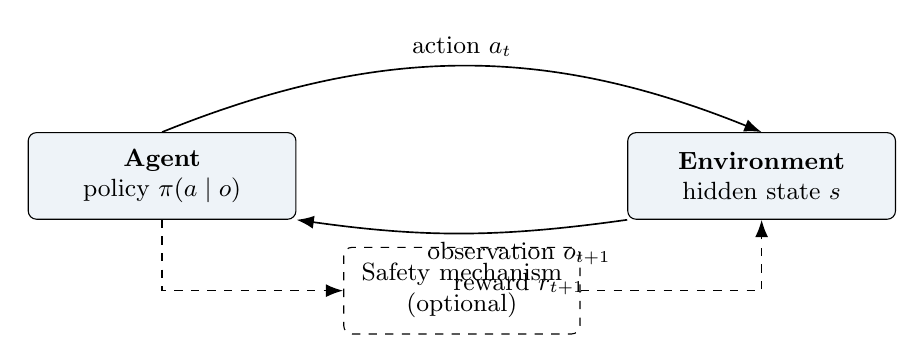
\begin{tikzpicture}[font=\small, box/.style={draw, rounded corners=3pt, fill=notebg, minimum width=3.4cm, minimum height=1.1cm, align=center}, arr/.style={-{Latex[length=2.2mm]}, line width=0.6pt}]
  \node[box] (agent) {\textbf{Agent}\\policy $\pi(a \mid o)$};
  \node[box, right=4.2cm of agent] (env) {\textbf{Environment}\\hidden state $s$};
  \node[box, fill=white, dashed, below=0.9cm of $(agent)!0.5!(env)$, minimum width=3cm] (shield) {Safety mechanism\\(optional)};
  \draw[arr] (agent.north) to[bend left=22] node[above] {action $a_t$} (env.north);
  \draw[arr] (env.south west) to[bend left=8] node[below, pos=0.35, xshift=4pt] {\shortstack{observation $o_{t+1}$\\reward $r_{t+1}$}} (agent.south east);
  \draw[arr, dashed] (agent.south) |- (shield.west);
  \draw[arr, dashed] (shield.east) -| (env.south);
\end{tikzpicture}
\caption{The agent--environment loop. The agent never sees the hidden state, only observations. A safety mechanism, where present, sits between the agent's choice and its execution.}
\label{fig:loop}
\end{figure}

%======================================================================
\section{The Mathematics Behind an Environment}

\subsection{Markov decision processes}
The standard model of an environment is the \textbf{Markov decision process} (MDP), a tuple $(S, A, P, R, \gamma)$~\cite{sutton}:
\begin{itemize}
  \item $S$, the set of \textbf{states}: everything that matters about the situation.
  \item $A$, the set of \textbf{actions} the agent can take.
  \item $P(s' \mid s, a)$, the \textbf{transition} probabilities: where an action leads.
  \item $R(s, a, s')$, the \textbf{reward}: an immediate number for each transition.
  \item $\gamma \in [0, 1]$, the \textbf{discount}: how much later rewards count relative to immediate ones.
\end{itemize}
The word \emph{Markov} means that the current state contains everything needed to predict what happens next; the history adds nothing. This property matters in practice: if the observation you give the agent is not Markov, a feed-forward network cannot learn a good policy from it.

\subsection{Return, policy and value}
The agent tries to maximise the \textbf{return}, the discounted sum of future rewards from step $t$:
\begin{equation}
G_t = r_{t+1} + \gamma\, r_{t+2} + \gamma^2 r_{t+3} + \dots = \sum_{k=0}^{T-t-1} \gamma^k\, r_{t+k+1}.
\end{equation}
A \textbf{policy} $\pi(a \mid s)$ gives the probability of each action in each state. The \textbf{action value} $Q^\pi(s, a)$ is the expected return from taking action $a$ in state $s$ and following $\pi$ afterwards. The optimal action values satisfy the \textbf{Bellman optimality equation}:
\begin{equation}
Q^*(s, a) = \mathbb{E}\big[\, r + \gamma \max_{a'} Q^*(s', a') \;\big|\; s, a \big].
\label{eq:bellman}
\end{equation}
Value-based methods such as Q-learning and the deep Q-network (DQN)~\cite{mnih} learn $Q$ by repeatedly nudging their estimate towards the right-hand side of Equation~\eqref{eq:bellman}. Once $Q$ is known, the policy is simply ``take the action with the highest $Q$''. Notice the $\max_{a'}$: it is the reason invalid actions must also be excluded from the learning target, not only from action selection (Section~\ref{sec:masking}).

\subsection{Partial observability}
In many real problems the agent cannot see the state. A doctor does not see the disease, only symptoms and test results; an IT technician does not see the cause of an incident, only error messages and check results. This is a \textbf{partially observable} MDP (POMDP)~\cite{kaelbling}: the agent receives an \textbf{observation} $o$ drawn from $O(o \mid s)$ instead of $s$ itself.

In a POMDP the agent should act on its \textbf{belief}, the probability distribution over hidden states given everything observed so far. With a hidden cause $c$ and observed evidence $e_1, \dots, e_n$ that are independent given the cause, Bayes' rule gives
\begin{equation}
b(c) = P(c \mid e_1, \dots, e_n) \;\propto\; P(c) \prod_{i=1}^{n} P(e_i \mid c).
\label{eq:belief}
\end{equation}
There are two ways to build an agent for a POMDP. One is to compute the belief explicitly and act on it; this is what the threshold baseline of this project does. The other is to give the agent an observation that \emph{summarises the evidence} and let a neural network learn to act on it; this is what the DQN agent does. The second works only if the summary is sufficient, which is why the design of the observation (Section~\ref{sec:obs}) matters so much.

\keypoint{An environment is an MDP or POMDP written as code. Every choice you make in code (what goes in the observation, what the actions are, what the reward pays for, when an episode ends) is a choice of $S$, $A$, $P$, $R$ and $\gamma$.}

%======================================================================
\section{The Six Design Decisions}

Every environment answers six questions. Table~\ref{tab:decisions} lists them with the answers this project gives. The rest of the manual explains how to answer each one well.

\begin{table}[h]
\centering\small
\caption{The six design decisions of an environment.}
\label{tab:decisions}
\begin{tabularx}{\textwidth}{@{}p{2.6cm}LL@{}}
\toprule
Decision & Question & This project \\
\midrule
Hidden state & What is true but unseen? & The cause of the incident; all check results \\
Observation & What can the agent see, and how is it encoded? & Status of each check, symptoms, context, step count, blocked flag \\
Actions & What can the agent do? & Run one of 20 checks, recommend one of about 15 fixes, escalate \\
Transitions & What happens after each action? & A check reveals its result; a fix or escalation ends the episode \\
Reward & What counts as good? & $+$ correct fix; $-$ wrong fix; $-$ check cost; $-$ escalation \\
Episode end & When does it stop? & Fix, escalation, forced escalation, or the step limit \\
\bottomrule
\end{tabularx}
\end{table}

%======================================================================
\section{Gymnasium: The Standard Interface}

\textbf{Gymnasium} is the maintained successor to OpenAI Gym and the standard interface for RL environments in Python~\cite{gymnasium}. If an environment follows it, any compatible library (Stable-Baselines3, sb3-contrib, RLlib, CleanRL) can train on it without changes. An environment is a class that inherits from \texttt{gymnasium.Env} and provides the members in Table~\ref{tab:api}.

\begin{table}[h]
\centering\small
\caption{The Gymnasium environment interface (version 1.x).}
\label{tab:api}
\begin{tabularx}{\textwidth}{@{}p{4.1cm}L@{}}
\toprule
Member & Purpose \\
\midrule
\texttt{action\_space} & The set of valid actions, as a \texttt{Space} object. Set in \texttt{\_\_init\_\_}. \\
\texttt{observation\_space} & The shape, type and bounds of observations. Set in \texttt{\_\_init\_\_}. \\
\texttt{reset(seed, options)} & Starts a new episode. Returns \texttt{(observation, info)}. Must call \texttt{super().reset(seed=seed)} first, which seeds \texttt{self.np\_random}. \\
\texttt{step(action)} & Applies one action. Returns \texttt{(observation, reward, terminated, truncated, info)}. \\
\texttt{render()} & Optional. Shows the current state, for debugging or demonstration. \\
\texttt{close()} & Optional. Releases resources such as windows or files. \\
\texttt{metadata} & Class attribute, e.g.\ the supported \texttt{render\_modes}. \\
\bottomrule
\end{tabularx}
\end{table}

\subsection{Spaces}
Spaces describe what valid actions and observations look like. The common ones are:
\begin{itemize}
  \item \texttt{Discrete(n)}: integers $0, \dots, n-1$. The usual action space for choosing one of $n$ options. DQN supports only this kind of action space.
  \item \texttt{Box(low, high, shape, dtype)}: real-valued arrays with bounds. The usual observation space. A flat \texttt{Box} works with the standard \texttt{"MlpPolicy"}.
  \item \texttt{MultiBinary(n)}, \texttt{MultiDiscrete([n1, n2, ...])}: vectors of binary or integer values.
  \item \texttt{Dict} and \texttt{Tuple}: combinations of other spaces. They need \texttt{"MultiInputPolicy"} in Stable-Baselines3; a single flat \texttt{Box} is simpler.
\end{itemize}
Every observation returned by \texttt{reset} and \texttt{step} must lie in \texttt{observation\_space}, with the same \texttt{dtype} (usually \texttt{np.float32}). A mismatch is the most common error that the environment checker reports.

\subsection{The two ways an episode ends}
\label{sec:endings}
Gymnasium distinguishes two endings, and the difference changes what the agent learns~\cite{pardo}:
\begin{itemize}
  \item \texttt{terminated=True}: the episode reached a \emph{true end of the task}, such as a fix being applied. There is no future, so the learning target is just the final reward.
  \item \texttt{truncated=True}: the episode was \emph{cut off for reasons outside the task}, such as a time limit imposed only to keep training runs short. The task would have continued, so the learner should still bootstrap from the value of the next state.
\end{itemize}
If a time limit is part of the problem, and the agent can see how much time remains, then reaching it is a termination. In this project the step limit is part of the task (reaching it means the incident is escalated, at a cost) and the step count is in the observation, so it is a termination. Treating it as truncation would teach the agent that stalling is free.

\subsection{Seeding and randomness}
All randomness inside an environment must come from \texttt{self.np\_random}, the generator that \texttt{super().reset(seed=seed)} creates. Never use Python's \texttt{random} module or \texttt{np.random} directly inside an environment. With this rule, \texttt{reset(seed=7)} always produces the same incident, which makes bugs reproducible and allows every policy to be evaluated on exactly the same incidents.

\subsection{Wrappers and registration}
A \textbf{wrapper} is an object that wraps an environment and changes one aspect of it without editing it: \texttt{ObservationWrapper} changes observations, \texttt{RewardWrapper} changes rewards, \texttt{ActionWrapper} changes actions. Stable-Baselines3's \texttt{Monitor} wrapper records episode returns and lengths. Wrappers are how you add things that differ between experiments (for example, an extra penalty for the penalty-only baseline) without making copies of the environment. \textbf{Registration} lets the environment be created by name. It is optional but convenient:
\begin{lstlisting}[numbers=none]
gymnasium.register(id="Triage-v0", entry_point="triage.env:TriageEnv")
env = gymnasium.make("Triage-v0")
\end{lstlisting}

%======================================================================
\section{A Worked Example: A Toy Triage Environment}
\label{sec:toy}

The best way to understand an environment is to build a small one completely. Listing~\ref{lst:toy} is a toy version of this project's environment: three hidden causes, two checks with different costs, three fixes and one escalate action. The likelihood matrix \texttt{theta} says how often each check is positive under each cause. Check 0 is good at recognising cause 0, check 1 is good at recognising cause 1, and cause 2 is ambiguous on both: this is deliberate, so that the agent has a reason to escalate.

\lstinputlisting[caption={A complete toy triage environment (\texttt{code/toy\_triage\_env.py}).}, label={lst:toy}]{code/toy_triage_env.py}

Read the listing with Section~\ref{sec:design} beside it. Four details deserve attention now:
\begin{itemize}
  \item \textbf{Lines 35--40} build the observation as a one-hot vector: for each check, exactly one of \emph{not requested}, \emph{negative}, \emph{positive} is 1.
  \item \textbf{Line 52} draws every check result once at the start of the episode. Running a check twice therefore gives the same answer, as it would in reality, and the observation stays Markov.
  \item \textbf{Lines 42--45} define \texttt{action\_masks()}: checks already run are unavailable. Learners that support masking will never choose them.
  \item \textbf{Lines 73--75} implement the step limit as a forced escalation that costs the agent the escalation penalty, and they return \texttt{terminated=True} for the reason given in Section~\ref{sec:endings}.
\end{itemize}

%======================================================================
\section{Design Decisions in Depth}
\label{sec:design}

\subsection{Observations}
\label{sec:obs}
The observation must contain everything the agent needs to act well, encoded so that a network can use it.

\textbf{Sufficiency.} Ask: could a perfect decision-maker act optimally from this observation alone? In triage, the results of the checks so far, the symptoms and the context are sufficient, because check results do not change during an episode. The step count is also needed, because the value of running another check depends on how many steps remain.

\textbf{Encoding.} Use \textbf{one-hot encoding} for categories. Encoding a check's status as $0, 1, 2$ in a single number would tell the network that ``positive'' is twice ``negative'', which is meaningless; three separate 0/1 entries carry no such false order. Scale numbers to roughly $[0, 1]$ (divide the step count by the step limit), because networks learn poorly from inputs of very different sizes.

\textbf{What not to include.} Never put the hidden state (the true cause) or anything computed from it into the observation. This is \textbf{information leakage}, and it produces agents that look perfect and are worthless. The toy environment returns the cause in the \texttt{info} dictionary for testing and logging only; learners do not read \texttt{info}.

\subsection{Actions and action masking}
\label{sec:masking}
A \texttt{Discrete} action space with a fixed numbering is simplest: in the toy, actions 0--1 are checks, 2--4 are fixes, 5 is escalate. In this project, with 20 checks and 15 causes, actions 0--19 are checks, 20--34 are fixes and 35 is escalate: $20 + 15 + 1 = 36$.

Some actions are \textbf{invalid} in some states, such as repeating a check. There are three ways to handle this~\cite{huang}:
\begin{enumerate}
  \item \textbf{Penalise} invalid actions with a negative reward. Simple, but the agent wastes training time learning what is invalid, and it may still choose invalid actions.
  \item \textbf{Ignore} them: treat an invalid action as a wasted step. Safe, but just as slow to learn.
  \item \textbf{Mask} them: the learner is told which actions are valid and never chooses the others. This is the most efficient, and Huang and Onta\~n\'on show that it scales to large action spaces where penalties fail~\cite{huang}.
\end{enumerate}
Masking must be applied in two places for value-based learners: in \emph{choosing} the action, and in the $\max_{a'}$ of the learning target (Equation~\ref{eq:bellman}). Otherwise the agent learns values that assume it can take actions it cannot. Section~\ref{sec:learners} shows both.

\keypoint{Do not mask actions that the \emph{rules} forbid before the agent proposes them. If rule-forbidden fixes were masked in advance, the agent could never propose a violation, and the study could not measure whether it learns the rules. In this project only repeated checks are masked in advance; rule violations are caught by the safety mechanism \emph{after} the proposal, and the blocked action is masked only for the agent's second try.}

The environment must still behave sensibly if an invalid action arrives, because some code paths (random exploration in libraries without masking, your own tests) will send one. In the toy, a repeated check simply returns the same result and costs the check again.

\subsection{Rewards}
The reward is the only way to tell the agent what you want. Three principles apply.

\textbf{Reward outcomes, not methods.} Pay for a correct fix and charge for costs; do not pay the agent for ``running the right check'', because you would be imposing your own strategy and the agent might learn to collect check rewards instead of resolving incidents. This failure, where an agent maximises the reward without doing the task, is called \textbf{reward hacking}. If extra guidance is needed, \textbf{potential-based shaping}, a reward of the form $\gamma\,\Phi(s') - \Phi(s)$ for some function $\Phi$ of the state, is the one form proven not to change which policy is optimal~\cite{ng}.

\textbf{The reward values encode a decision threshold.} Suppose the agent stops investigating and its belief that the most likely cause is correct is $p$. Recommending that fix has expected reward $p\, r_{\text{correct}} - (1-p)\,\lambda_{\text{wrong}}$; escalating has reward $-\lambda_{\text{esc}}$. Recommending is better exactly when
\begin{equation}
p \;>\; p^* = \frac{\lambda_{\text{wrong}} - \lambda_{\text{esc}}}{r_{\text{correct}} + \lambda_{\text{wrong}}}.
\label{eq:threshold}
\end{equation}
With the starting values $r_{\text{correct}} = 10$, $\lambda_{\text{wrong}} = 10$ and $\lambda_{\text{esc}} = 3$, the threshold is $p^* = 7/20 = 0.35$: the optimal agent will recommend a fix it believes is only 35\% likely to be right. That is probably too bold for IT operations. Raising the cost of a wrong fix to 20 gives $p^* = 17/30 \approx 0.57$; raising it to 40 gives $p^* = 37/50 = 0.74$. Equation~\eqref{eq:threshold} turns the abstract question ``what should the rewards be?'' into a concrete one that the Directorate can answer: \emph{how sure should someone be before applying a fix rather than escalating?}

The toy environment makes the effect visible. Because it is tiny, its exact optimal policy can be computed by searching every possible sequence of check results (\texttt{code/optimal\_toy.py}). Table~\ref{tab:threshold} shows that optimal policy for three costs of a wrong fix, all else equal. With $\lambda_{\text{wrong}} = 10$ the best possible agent \emph{never} escalates and is wrong 28\% of the time; it is not misbehaving, it is doing exactly what the rewards ask. As a wrong fix becomes more costly, the optimal agent escalates more and errs less.

\begin{table}[h]
\centering\small
\caption{Optimal behaviour of the toy environment as the cost of a wrong fix rises ($r_{\text{correct}} = 10$, $\lambda_{\text{esc}} = 3$; outcome shares over 1{,}000 incidents).}
\label{tab:threshold}
\begin{tabular}{@{}rrrrrr@{}}
\toprule
$\lambda_{\text{wrong}}$ & $p^*$ & Optimal return & Correct & Wrong & Escalated \\
\midrule
10 & 0.35 & 4.20 & 71.9\% & 28.1\% & 0.0\% \\
20 & 0.57 & 1.85 & 67.2\% & 20.3\% & 12.5\% \\
40 & 0.74 & -0.50 & 57.6\% & 10.9\% & 31.5\% \\
\bottomrule
\end{tabular}

\end{table}

\textbf{Check costs set how much evidence is worth buying.} A check is worth running only if the expected improvement in the final decision exceeds its cost. If checks are free, the agent will run all of them; if they are expensive relative to the threshold, it will run none. Pilot runs should confirm that the agent runs some checks, and fewer when the evidence is already clear.

\textbf{Scale and discount.} Keep rewards roughly in $[-50, 50]$; very large values destabilise learning. Episodes here are short and the check costs already penalise delay, so $\gamma = 0.99$ (the library default) or $\gamma = 1$ both work. Report the choice.

\subsection{Episode structure}
Every episode must end. Give each one an explicit step limit and test that it is reached (Listing~\ref{lst:tests}). Decide for each ending whether it is a termination or a truncation (Section~\ref{sec:endings}), and record the reason in \texttt{info} (\texttt{"outcome"} in the toy) so that the evaluation can count correct fixes, wrong fixes, escalations and step-limit escalations separately.

\subsection{Randomness and controlled difficulty}
A simulator is valuable because its difficulty can be controlled. In the toy, randomness enters at \texttt{reset}: the cause is drawn from the prior and the check results from \texttt{theta}. Difficulty controls are parameters of the constructor that change those draws. This project has three:
\begin{itemize}
  \item \textbf{Missing evidence} ($p_{\text{miss}}$): at \texttt{reset}, mark each check as unavailable with this probability. Running it returns \emph{unavailable}, a fourth status in the one-hot encoding.
  \item \textbf{Unreliable evidence} ($p_{\text{noise}}$): at \texttt{reset}, flip each drawn result with this probability.
  \item \textbf{Overlapping evidence} ($\omega$): in \texttt{\_\_init\_\_}, blend each cause's column of \texttt{theta} towards its category average, $\theta'_{ij} = (1-\omega)\,\theta_{ij} + \omega\,\bar\theta_i$.
\end{itemize}
Passing these through \texttt{reset(options=\{...\})} instead allows a different difficulty in every episode, which is how the randomised training regime is implemented.

\subsection{Constraints and the safety mechanism}
\label{sec:shield}
A \textbf{shield} is a component that checks each action against rules and prevents violations~\cite{shield}. There are two places to put it:
\begin{itemize}
  \item \textbf{As a wrapper} around the environment. Clean when the shield only replaces actions, but awkward when the agent must \emph{see} that it was blocked.
  \item \textbf{Inside \texttt{step}}, behind a constructor switch. Simpler when the shield changes the observation (the \emph{blocked} flag) and the mask.
\end{itemize}
This project uses the second. In \texttt{step}, before executing an action: (1) evaluate the rules; (2) if the action is permitted, execute it; (3) if it is forbidden and this is the first block, do not execute it, set the blocked flag, mask that action, give zero reward and return; (4) if it is a second consecutive block, end the episode as a \emph{forced escalation}. The rules themselves should be data (a list loaded from a configuration file) evaluated by a small function such as \texttt{is\_forbidden(action, context, evidence)}, so that they can be read and reviewed without reading the agent's code. A switch \texttt{shield=False} produces the unconstrained baseline, and a wrapper that subtracts a penalty for each violation produces the penalty-only baseline, from the same environment class.

%======================================================================
\section{Connecting a Learner}
\label{sec:learners}

\textbf{Stable-Baselines3} (SB3) provides tested implementations of the standard algorithms~\cite{sb3}, and \textbf{sb3-contrib} adds \texttt{MaskablePPO}, a PPO that accepts action masks. SB3's \texttt{DQN} does not support masks, so Listing~\ref{lst:dqn} extends it. The environment appends its mask to the end of the observation (a small \texttt{ObservationWrapper} does this). The Q-network then sets the value of every masked action to a very large negative number. Because the target network also reads the mask from the \emph{next} observation, this one change covers both action selection and the $\max$ in the learning target. Two further overrides make random exploration respect the mask.

\lstinputlisting[caption={DQN with action masking (\texttt{code/masked\_dqn.py}).}, label={lst:dqn}]{code/masked_dqn.py}

Training and evaluation then take a few lines (Listing~\ref{lst:train}); each run takes one to three minutes on a laptop CPU. Note \texttt{net\_arch=[128, 128]}, the two hidden layers of 128 units chosen for this project; the evaluation seeds start at 10{,}000 so that the agent is evaluated on incidents it never trained on.

\lstinputlisting[caption={Training both learners on the toy environment (excerpt of \texttt{code/train\_toy.py}).}, label={lst:train}, firstline=37, lastline=49, firstnumber=37]{code/train_toy.py}

\textbf{Monitoring training.} Wrap the training environment in \texttt{Monitor} and watch the mean episode return. It should rise and then level off. If it never rises, suspect the environment or the reward before the hyperparameters. SB3's \texttt{EvalCallback} evaluates the agent on a separate environment every few thousand steps and saves the best model.

%======================================================================
\section{Testing an Environment}
\label{sec:testing}

Test the environment before training any agent on it. Listing~\ref{lst:tests} shows the five tests used for the toy; each catches a different class of bug.

\lstinputlisting[caption={Tests for the toy environment (\texttt{code/test\_toy\_env.py}).}, label={lst:tests}]{code/test_toy_env.py}

\begin{enumerate}
  \item \textbf{API conformance.} Gymnasium's \texttt{check\_env} confirms that spaces, data types, return values and seeding follow the interface.
  \item \textbf{Determinism.} The same seed must give the same incident. Without this no result can be reproduced.
  \item \textbf{Statistical correctness.} Over many episodes, the frequency of each cause must match the prior and the frequency of positive checks must match \texttt{theta}. This catches indexing errors (rows and columns swapped), which are otherwise invisible.
  \item \textbf{Reward ordering.} The configured rewards must satisfy $r_{\text{correct}} > -\lambda_{\text{esc}} > -\lambda_{\text{wrong}}$.
  \item \textbf{Termination.} Every episode must end, even for an agent that repeats one action forever.
\end{enumerate}

Then run \textbf{reference policies} and check their scores make sense before training. A \emph{random} policy gives a floor. An \emph{always-escalate} policy gives exactly $-\lambda_{\text{esc}}$ per episode. An \emph{oracle} that is told the cause gives $r_{\text{correct}}$; no agent that cannot see the cause can reach it, so an agent that comes close has almost certainly been given leaked information. In a small environment the \emph{exact optimum} can be computed and is the true ceiling. In the project environment, with $4^{20}$ possible check histories, it cannot, and the \emph{threshold} policy, which computes the belief of Equation~\eqref{eq:belief} and acts when it is confident, serves as a strong reference instead. It is a heuristic, not a ceiling: a learned agent can beat it.

\textbf{Results on the toy.} Table~\ref{tab:toyresults} shows every policy on the same 1{,}000 unseen incidents. Both learners reach the exact optimum, which confirms that the environment, the masking and the training code work together. Two lessons carry over to the project. First, the threshold heuristic falls short of the optimum because its fixed confidence rule (act above 0.8) is not what the rewards ask for, which is why it is a reference and not a ceiling. Second, the masked DQN needed about 100{,}000 steps; at 30{,}000 it still escalated 39\% of incidents and scored 1.77, while PPO converged in 30{,}000. Training length must be set from learning curves, not guessed. These are checks of the toy, not results of this project.

\begin{table}[h]
\centering\small
\caption{All policies on the toy environment, 1{,}000 unseen incidents (\texttt{code/make\_toy\_results.py}).}
\label{tab:toyresults}
\begin{tabular}{@{}lrrrrr@{}}
\toprule
Policy & Mean return & Correct & Wrong & Escalated & Step limit \\
\midrule
Random (valid actions) & -3.32 & 25.1\% & 49.2\% & 25.7\% & 0.0\% \\
Always escalate & -3.00 & 0.0\% & 0.0\% & 100.0\% & 0.0\% \\
Threshold (knows $\theta$) & 3.68 & 71.9\% & 28.1\% & 0.0\% & 0.0\% \\
Masked DQN (100k steps) & 4.18 & 71.9\% & 28.1\% & 0.0\% & 0.0\% \\
MaskablePPO (30k steps) & 4.18 & 71.9\% & 28.1\% & 0.0\% & 0.0\% \\
Exact optimum & 4.18 & 71.9\% & 28.1\% & 0.0\% & 0.0\% \\
Oracle (told the cause) & 10.00 & 100.0\% & 0.0\% & 0.0\% & 0.0\% \\
\bottomrule
\end{tabular}

\end{table}

%======================================================================
\section{Common Mistakes}

\begin{tabularx}{\textwidth}{@{}p{4.2cm}L@{}}
\toprule
Mistake & Consequence and remedy \\
\midrule
Hidden state in the observation & Perfect but meaningless agent. Keep the cause in \texttt{info} only, and test that the observation does not change when only the cause changes. \\
Using \texttt{np.random} in the environment & Seeds have no effect; nothing is reproducible. Use \texttt{self.np\_random}. \\
Wrong \texttt{dtype} or bounds & \texttt{check\_env} fails or learning is silently wrong. Return \texttt{np.float32} within the declared bounds. \\
Time limit as truncation when it is part of the task & Agent learns that stalling is free. Use \texttt{terminated} and charge the cost. \\
Masking only action selection in DQN & Learning targets use impossible actions; values are overestimated. Mask inside the Q-network. \\
Masking rule-forbidden actions in advance & No violations can occur, so compliance cannot be measured. Mask only after a block. \\
Unchecked reward values & Agent is too bold or too timid. Compute the threshold of Equation~\eqref{eq:threshold} first. \\
Training and evaluating on the same seeds & Overstated results. Keep separate seed ranges. \\
Tuning the simulator after seeing the agent's results & The environment is fitted to the agent. Freeze the scenario model before training. \\
\bottomrule
\end{tabularx}

%======================================================================
\section{From This Manual to Our Environment}

The project's environment is the toy of Section~\ref{sec:toy} grown along the lines of Section~\ref{sec:design}. Table~\ref{tab:map} lists the differences.

\begin{table}[h]
\centering\small
\caption{From the toy environment to the project environment.}
\label{tab:map}
\begin{tabularx}{\textwidth}{@{}p{3.2cm}LL@{}}
\toprule
Element & Toy & Project \\
\midrule
Causes, checks & 3 causes, 2 checks, hard-coded & About 15 causes, 20 checks, loaded from the elicitation workbook \\
Check status & 3 values & 4 values (adds \emph{unavailable}) \\
Observation & Checks, step count & Adds symptoms (3 values each), context attributes, blocked flag, action mask \\
Actions & 6 & 36 \\
Ambiguity & None & $p_{\text{miss}}$, $p_{\text{noise}}$, $\omega$, fixed or drawn per episode \\
Rules & None & 10 rules from a configuration file, checked inside \texttt{step} \\
Reference labels & None & ``Should escalate'' label in \texttt{info}, for evaluation only \\
\bottomrule
\end{tabularx}
\end{table}

\textbf{Package layout.} The code will be organised as follows, so that the scenario and rules are data and every experiment can be traced to its configuration:
\begin{lstlisting}[language={}, numbers=none]
triage/
  config/   scenario.yaml  rules.yaml  experiments/*.yaml
  scenario.py    # reads the workbook export -> prior, theta, symptom likelihoods, costs
  rules.py       # Rule objects and is_forbidden(action, context, evidence)
  env.py         # TriageEnv(gymnasium.Env): reset, step, action_masks, shield switch
  wrappers.py    # MaskInObservation, PenaltyOnly
  baselines.py   # initial-symptom, scripted, always-escalate, threshold
  masked_dqn.py  # Listing 2
  train.py  evaluate.py
tests/      test_env.py  test_rules.py  test_baselines.py
\end{lstlisting}

\textbf{Build order.} Each step is tested before the next begins:
\begin{enumerate}
  \item \textbf{Provisional scenario.} Write \texttt{scenario.yaml} by hand with invented values in the four categories, so that development does not wait for the elicitation. Replace it after the session.
  \item \textbf{Core environment.} Hidden cause, checks, symptoms, context, rewards and the step limit; pass the five tests of Listing~\ref{lst:tests}.
  \item \textbf{Ambiguity controls.} Add $p_{\text{miss}}$, $p_{\text{noise}}$ and $\omega$; test that each changes the statistics as intended.
  \item \textbf{Reference policies.} Random, always-escalate, oracle and threshold; check their scores are ordered as in Section~\ref{sec:testing}.
  \item \textbf{Rules and shield.} Implement \texttt{rules.py} and the review-then-escalate logic; test each rule with a hand-built incident.
  \item \textbf{Learners.} Train the masked DQN on the provisional scenario as a smoke test; only then on the frozen elicited scenario.
\end{enumerate}

%======================================================================
\begin{thebibliography}{9}\small
\bibitem{sutton} R.~S. Sutton and A.~G. Barto, \emph{Reinforcement Learning: An Introduction}, 2nd~ed. Cambridge, MA, USA: MIT Press, 2018.
\bibitem{kaelbling} L.~P. Kaelbling, M.~L. Littman, and A.~R. Cassandra, ``Planning and acting in partially observable stochastic domains,'' \emph{Artificial Intelligence}, vol.~101, no.~1--2, pp.~99--134, 1998.
\bibitem{gymnasium} M.~Towers \emph{et al.}, ``Gymnasium: A standard interface for reinforcement learning environments,'' arXiv:2407.17032, 2024.
\bibitem{sb3} A.~Raffin \emph{et al.}, ``Stable-Baselines3: Reliable reinforcement learning implementations,'' \emph{Journal of Machine Learning Research}, vol.~22, no.~268, pp.~1--8, 2021.
\bibitem{pardo} F.~Pardo, A.~Tavakoli, V.~Levdik, and P.~Kormushev, ``Time limits in reinforcement learning,'' in \emph{Proc. 35th Int. Conf. Machine Learning (ICML)}, 2018, pp.~4045--4054.
\bibitem{huang} S.~Huang and S.~Onta\~n\'on, ``A closer look at invalid action masking in policy gradient algorithms,'' in \emph{Proc. 35th Int. FLAIRS Conf.}, 2022.
\bibitem{ng} A.~Y. Ng, D.~Harada, and S.~Russell, ``Policy invariance under reward transformations: Theory and application to reward shaping,'' in \emph{Proc. 16th Int. Conf. Machine Learning (ICML)}, 1999, pp.~278--287.
\bibitem{shield} M.~Alshiekh, R.~Bloem, R.~Ehlers, B.~K\"onighofer, S.~Niekum, and U.~Topcu, ``Safe reinforcement learning via shielding,'' in \emph{Proc. AAAI Conf. Artificial Intelligence}, vol.~32, no.~1, 2018.
\bibitem{mnih} V.~Mnih \emph{et al.}, ``Human-level control through deep reinforcement learning,'' \emph{Nature}, vol.~518, no.~7540, pp.~529--533, 2015.
\end{thebibliography}

\end{document}
